\section{Regular-patch derivatives and the quotient model}\label{sec:derivatives}

\subsection{Preserving the quadratic rate in holomorphic coordinates}
The direct spectral proof in section~\ref{sec:scattering} controls the
selected curvature uniformly in $b/a$. A complementary approach on
regular angular patches upgrades \eqref{eq:metriccomparison} to metric
derivative estimates. Its quadratic rate cannot simply be differentiated;
the additional input is that both metrics are Ricci-flat K\"ahler in
the same complex structure.

\begin{lemma}\label{lem:interior}
Let $g_*$ be a smooth Ricci-flat K\"ahler metric on a complex manifold
$U$, and let $K\Subset U_1\Subset U$. Suppose $g_t$ are Ricci-flat
K\"ahler for the same complex structure and
$\sup_{U_1}|g_t-g_*|_{g_*}\le e_t\to0$. Then for every fixed
integer $k\ge0$ and $0<\alpha<1$,
\begin{equation}\label{eq:interior}
 \|g_t-g_*\|_{C^{k,\alpha}(K,g_*)}\le C_{K,U_1,g_*,k,\alpha}e_t
\end{equation}
for all sufficiently small $t$. The comparison uses the original
complex coordinates, without a parameter-dependent coordinate change.
\end{lemma}
\begin{proof}
Cover $K$ by finitely many fixed holomorphic coordinate balls compactly
contained in larger balls in $U_1$. Uniform metric equivalence and
\cite[Proposition~2.1]{hein_tosatti} give uniform bounds for every
fixed coordinate derivative on intermediate balls. These estimates
alone do not preserve the rate $e_t$.

For a Ricci-flat K\"ahler metric, differentiation of $\log\det g$
and the K\"ahler interchange of derivatives give
\begin{equation}\label{eq:RFsystem}
 g^{p\bar q}\partial_p\partial_{\bar q}g_{i\bar j}
 =g^{p\bar q}g^{r\bar s}
  (\partial_i g_{p\bar s})(\partial_{\bar j}g_{r\bar q}).
\end{equation}
Subtract the equations for $g_t$ and $g_*$, and write $h=g_t-g_*$.
The inverse difference is $g_*^{-1}-g_t^{-1}=g_t^{-1}hg_*^{-1}$.
Integrating the differential of the quadratic right side along
$g_*+sh$, $0\le s\le1$, gives a homogeneous linear system
\begin{equation}\label{eq:homogeneous}
 g_t^{p\bar q}\partial_p\partial_{\bar q}h
                      =A_t\cdot Dh+B_t h.
\end{equation}
$D$ here includes all real first derivatives. The principal symbol
is scalar times the identity on Hermitian components. Its ellipticity
and all needed coefficient norms are uniform on intermediate balls
by the preceding regularity estimate.

For clarity, lower-order coupling does not require a maximum
principle for a system. Apply scalar interior Schauder estimates
componentwise in the usual boundary-distance-weighted H\"older norms
on an intermediate ball. They give
\[
 |h|^*_{2,\alpha}\le C\|h\|_0+
 C_1\bigl(|h|^*_{1,\alpha}+|h|^*_{0,\alpha}\bigr).
\]
Weighted interpolation bounds the parenthesis by
$\delta |h|^*_{2,\alpha}+C_\delta\|h\|_0$.
Choose $C_1\delta<1/2$ and absorb. The weights are bounded below
on a smaller ball, yielding the ordinary $C^{2,\alpha}$ bound
by $\|h\|_0\le e_t$. Differentiating \eqref{eq:homogeneous}
and using nested balls gives each higher order inductively, since
every differentiated forcing term has the already established rate.
The finite cover proves \eqref{eq:interior}.
\end{proof}

Let $\delta_\varepsilon$ be cone dilation and put
\begin{equation}\label{eq:rescaled}
 g_\varepsilon=\varepsilon^{-2}\delta_\varepsilon^*\Psi^*\gKS.
\end{equation}
On any compact subset $K$ of the smooth-simple annulus
$\Cone\cap\{1/4<r<4\}$, both $g_\varepsilon$ and $\gC$ are
Ricci-flat K\"ahler in the same holomorphic chart. Equation
\eqref{eq:metriccomparison}, on a slightly larger regular neighborhood,
and Lemma~\ref{lem:interior} give
\begin{equation}\label{eq:all-derivatives}
 \|g_\varepsilon-\gC\|_{C^{k,\alpha}(K,\gC)}
                         \le C_{K,k,\alpha}\varepsilon^2.
\end{equation}
This is a standard elliptic consequence of the imported quadratic
comparison, not a new general regularity theorem.

The dependence on the smooth chart can also be made explicit.
Call a holomorphic embedding
$\varphi:B_{\CC^n}(0,2)\to\Cone_{\rm simple}$ admissible at
scale $0<\rho\le1$ if its image lies in $1/4<r<4$ and
\begin{equation}\label{eq:chartscale}
 \Lambda^{-1}g_{\rm Eucl}\le\rho^{-2}\varphi^*\gC
                                     \le\Lambda g_{\rm Eucl}
\end{equation}
for a fixed $\Lambda$. Apply the same proof to the two pulled-back
metrics divided by $\rho^2$. The reference derivatives are uniformly
bounded by the same local Ricci-flat estimate, so at the chart center
\begin{align}\label{eq:weighted}
 |\nabla^k(g_\varepsilon-\gC)|_{\gC}
   &\le C_k\varepsilon^2\rho^{-k},\\
 |\Rm(g_\varepsilon)-\Rm(\gC)|_{\gC}
   &\le C\varepsilon^2\rho^{-2}.\nonumber
\end{align}
Use the same tensor type on both sides of the curvature difference.
No lower bound for this admissible $\rho$ in terms of $b/a$ is
asserted. Such a lower bound, not merely the existence of very small
charts, would be needed to turn \eqref{eq:weighted} into an explicit
estimate uniform toward the Pauli axis.

\subsection{What fails near a changing stabilizer}
There is a direct diagnostic within the balanced locus. Add
$X_3=c\sigma_2$ to \eqref{eq:pauli}, with $a,b,c$ real and
$Y=0$. On the real two-plane of components
$(X_2\sigma_2,X_3\sigma_1)$, the orthogonal projection onto the
orbit of $i\sigma_3$ is
\begin{equation}\label{eq:projector}
 P(b,c)=\frac1{b^2+c^2}
 \begin{pmatrix}b^2&-bc\\-bc&c^2\end{pmatrix}.
\end{equation}
The other orbit generators occupy mutually orthogonal component
planes. At $c=0$,
\begin{equation}\label{eq:projectorderivatives}
 \partial_cP=\begin{pmatrix}0&-b^{-1}\\-b^{-1}&0\end{pmatrix},
 \qquad
 \partial_c^2P=\begin{pmatrix}-2b^{-2}&0\\0&2b^{-2}\end{pmatrix}.
\end{equation}
Their operator norms are $b^{-1}$ and $2b^{-2}$. Thus the
horizontal projection in the original balanced coordinates is not
uniformly $C^2$ as $b\to0$. This does not invalidate the relative
$C^0$ tensor comparison, and alone it is not an intrinsic curvature
calculation. The following calculation supplies the latter.

\subsection{Curvature in additional harmonic deformation directions}
At a Pauli point with $a,b>0$, let $u,v$ be the two Dolbeault
vectors in \eqref{eq:plane}. They are orthonormal for
\eqref{eq:flatmetric}. Their support is orthogonal to the orbit
and its three quaternionic images, so they are horizontal tangent
vectors to the hyperk\"ahler quotient.

\begin{proposition}\label{prop:curvature}
With curvature sign positive on a round sphere,
\begin{equation}\label{eq:conecurvature}
 K_{\gC}(u,v)=\frac3{2b^2}.
\end{equation}
For $a=\varepsilon$, $b=\kappa\varepsilon$ at fixed
$0<\kappa\le1$, transport this plane by $\Psi$ and normalize
using the actual harmonic metric. Its sectional curvature satisfies
\begin{equation}\label{eq:actualcurvature}
 K_{\gKS}=\frac3{2\kappa^2\varepsilon^2}+O_\kappa(1).
\end{equation}
\end{proposition}
\begin{proof}
The effective $\PU(2)$ action is free at this point and the moment
map is a submersion. Its zero set $N$ is a smooth submanifold of
the flat representation. Every tuple of Hermitian $X_j$ with
$Y=0$ lies in $N$. The affine plane $x+su+tv$ therefore lies
in $N$, and its three relevant second fundamental form entries
vanish. The Gauss equation gives $K_N(u,v)=0$.

Let $D_x\xi=([\xi,X_j],[\xi,Y_j])$ and use the bilinear
orbit Gram form $Q_x(\xi,\zeta)=\langle D_x\xi,D_x\zeta\rangle$,
viewed as a map from the Lie algebra to its dual. For horizontal
$u,v$, set $\beta(\xi)=\langle\xi\cdot u,v\rangle$.
Differentiating the one-form $\langle D_x\xi,\cdot\rangle$
gives $2\beta(\xi)$. Thus the curvature of the mechanical
connection is $2Q_x^{-1}\beta$, up to an irrelevant sign, and
the squared norm of O'Neill's tensor is $\beta(Q_x^{-1}\beta)$.
In the unnormalized basis $(i\sigma_1,i\sigma_2,i\sigma_3)$,
\begin{equation}\label{eq:orbitgram}
 Q_x=\operatorname{diag}(8a^2,8(a^2+b^2),8b^2),\qquad
 \beta=(0,0,-2).
\end{equation}
$Q_x$ here is the bilinear Gram matrix, not the matrix of
$D_x^*D_x$ after a Hilbert--Schmidt identification of the Lie
algebra with its dual. The resulting norm is $1/(2b^2)$.
O'Neill's formula \cite{oneill,bielawski} gives
$K_{N/\PU(2)}=K_N+3\|\mathcal A_{uv}\|^2$, proving
\eqref{eq:conecurvature}.

The ray with fixed $\kappa$ lies in a fixed regular angular patch;
its cone radius is $\sqrt{2(1+\kappa^2)}\varepsilon$.
The $C^2$ estimate \eqref{eq:all-derivatives} changes sectional
curvature of the rescaled metric by $O_\kappa(\varepsilon^2)$.
Scaling back gives \eqref{eq:actualcurvature}. In particular its
relative error is $O_\kappa(\varepsilon^2)$.
\end{proof}

Equation~\eqref{eq:actualcurvature} supplies an independent regular-ray
check of Proposition~\ref{prop:uniformcurvature}. The latter's direct
vertex proof also allows $b/a\to0$; the local derivative argument
above does not provide that additional uniformity. Section~\ref{sec:scalar}
identifies the leading physical coefficient while retaining the other
neutral fields.

\begin{figure}[t]
\centering
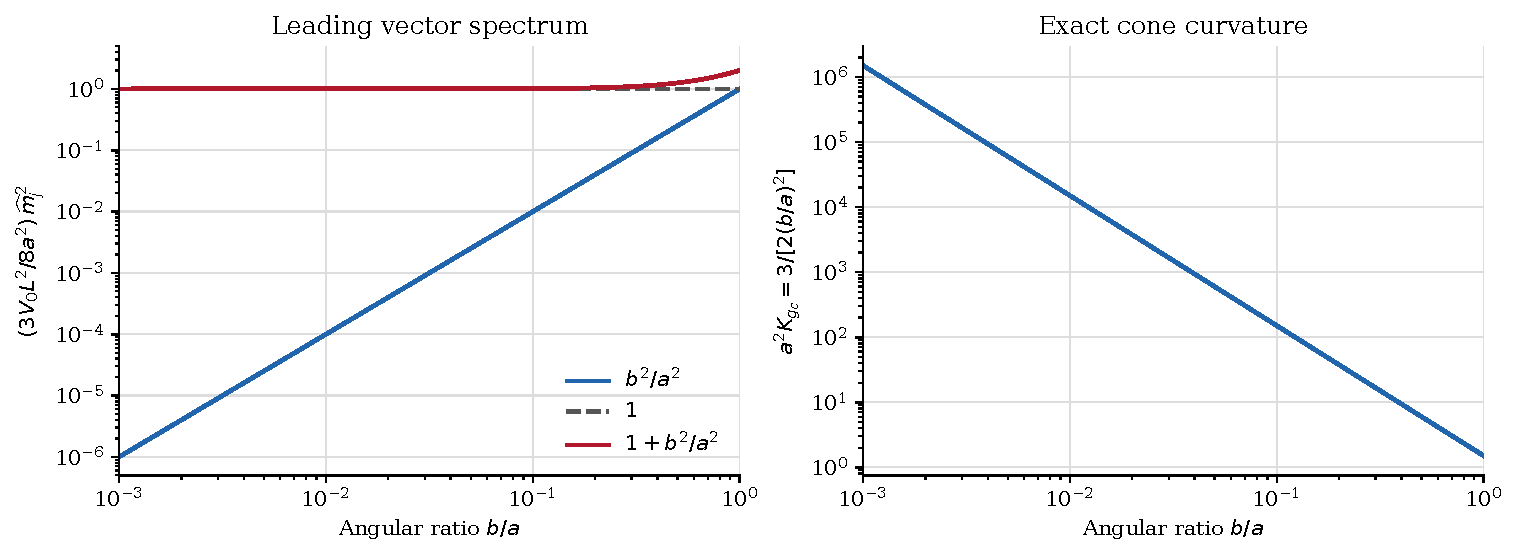
\includegraphics[width=\textwidth]{figures/output/finite_scales.pdf}
\caption{Exact finite-model formulas as the angular ratio decreases.
Left: the three normalized leading squared vector masses. The relative
geometric estimate remains uniform over the plotted ratios. Right:
the cone curvature of the horizontal two-plane \eqref{eq:plane}.
Proposition~\ref{prop:uniformcurvature} transfers this selected curvature
to the actual harmonic metric with uniform relative quadratic error for
$0<b\le\kappa_0a$, $\kappa_0<1$. Both panels
plot analytic formulas, not numerical HE solutions.}
\label{fig:scales}
\end{figure}
